% =====================================================================
%  第 5 章 Floer 同调（后半）—— ch05b
%  页段：PDF 227–252（原书 p.217–242）；§5.3 起 p.217，§5.4 起 p.229
%  含第 5 章章末评注
% =====================================================================

% [原文 p.217]
% 块首直接续 ch05a 末尾：p.216 末开始的 δ 的定义在 p.217 顶收尾，该分句已由 ch05a 写完，此处不再重复。
设 $M$ 为半正。

\begin{theorem}{5.74}
  （Hofer–Salamon、小野）$\delta\delta=0$ 成立。把 $HF(M;h)$ 取作 $(CF_k(M;f),\delta)$ 的同调，则
  \begin{equation}
    HF(M;h)\cong H(M;\Z)\otimes\Lambda_{\mathrm{nov},\Z}. \tag{5.13}
  \end{equation}
\end{theorem}
% [Tutor Note: 定理 5.74 里链复形写作 $(CF_k(M;f),\delta)$，但本节讨论的哈密顿函数是 $h$，同页下文也用 $h$，按定义 5.73 应作 $CF_k(M;h)$。译文照原书保留。]

$\delta\delta=0$ 由引理 5.72 得到。式 (5.13) 的证明将在下一节说明。对一般的 $M$，定理 5.74 的类似结论在 $\Q$ 系数下成立（[124], [237]）。

\begin{definition}{5.75}
  把 $HF(M;h)$ 称为周期哈密顿系统的 Floer 上同调。
\end{definition}

\section{Bott–Morse 理论再论}

本节概述下述结论的证明：$M$ 上周期哈密顿系统的 Floer 上同调，与 $M$ 的同调一致。大致说来，已知有两种做法。

\takeaway{本节用 Bott–Morse 理论把 Floer 同调与 $M$ 的同调对上：以谱序列 $E_2^k\cong\bigoplus_jH^{k-\mu(R_j)}(R_j;\Z)$ 为纲，用模空间 $\mathcal{M}(R_i,R_j;f)$ 的紧化与几何链写出微分，再证明同调不随 $f$ 改变。作者走方案 2，关键工具是上链映射 $\Phi^{f_\tau}$ 及其链同伦。}

\textbf{方案 1}
\begin{enumerate}[label=(\arabic*),leftmargin=2.4em,itemsep=1pt,topsep=2pt]
  \item 证明 Floer 同调不依赖于哈密顿函数 $h$。
  \item 其次，在 $h$ 不依赖于时间（$S^1$ 方向）、即 $h\colon M\to\R$ 的情形，并且 $h$ 充分小的情形，证明定义 Floer 同调的链复形与 $h$ 的 Morse–Witten 复形相同。
\end{enumerate}

\textbf{方案 2}
\begin{enumerate}[label=(\arabic*),leftmargin=2.4em,itemsep=1pt,topsep=2pt]
  \item 证明 Floer 同调不依赖于哈密顿函数 $h$。此时把假设放宽到 $h$ 的 1 周期解半非退化的情形，并在这一范围内证明 Floer 同调的定义与不变性。
  \item 在 $h=0$ 的情形计算 Floer 同调。
\end{enumerate}

许多文献的证明，例如 [103], [106], [124], [183], [293]，都采用方案 1。[117] 则在规范理论的 Floer 同调情形，执行了相当于方案 2 的构造。与此独立，Piunikhin 用方案 2 提出了计算 Floer

% [原文 p.218]
同调的方案\footnote{按方案 2 证明，还作为副产品得到关于积结构的定理，即量子杯积与 Floer 同调的积一致。}。基于方案 2 的证明在 [302], [318] 中预告过，但至今尚未发表。下面按方案 2、基于 [117] 的方法概述证明。

方案 2 的第 (1) 条，在有限维情形就是定理 3.17；第 (2) 条则是定理 3.23（其中的 $A$ 是动量映射）。因此本节省略关于无限维的诸问题（上一节已述及若干）的讨论，只叙述定理 3.17 与定理 3.23 的证明。不过，本节的证明与第 3 章的证明不同，可以推广到无限维情形。

设 $f\colon X\to\R$ 是有限维流形 $X$ 上的 Bott–Morse 函数。沿用定义 5.20 的记号。我们来构造定理 3.17，即谱序列
\[
E_2^k\simeq\bigoplus_{\mu(R_i)+j=k}H^j(R_i;\Z)\Longrightarrow H^k(X;\Z)
\]
的构造。与第 3 章定理 3.17 的证明不同之处在于：只使用模空间 $\mathcal{M}(R_i,R_j;f)$ 的语言，不用稳定流形等来构造。

\begin{definition}{5.76}
  用 $\ev_{\pm;i,j}([\gamma])=\gamma(\pm\infty)$ 定义 $\ev_{-;i,j}\colon\mathcal{M}(R_i,R_j;f)\to R_i$ 与 $\ev_{+;i,j}\colon\mathcal{M}(R_i,R_j;f)\to R_j$。
\end{definition}

\begin{lemma}{5.77}
  在临界点之外把 $f$ 稍作扰动，可使 $\ev_\pm$ 成为光滑映射。
\end{lemma}

证明见 [117]。

从式 (5.14) 这样的对应（correspondence）可以构造谱序列的微分，这是主要的想法。不准确地说，谱
\begin{equation}
\begin{array}{ccc}
  & \mathcal{M}(R_i,R_j;f) & \\[6pt]
  \swarrow_{\scriptstyle \ev_{-,i,j}} & & \searrow^{\scriptstyle \ev_{+,i,j}}\\[16pt]
  R_i & & R_j
\end{array}
\tag{5.14}
\end{equation}
% [Tutor Note: 式 (5.14) 是“对应”而非通常的交换图：两条斜向求值映射把模空间投到两个临界子流形，谱序列的微分正是由这个对应给出的，故图中不必加交换性假设。]

% [原文 p.219]
序列的微分，对 $R_i$ 的链 $P$ 由下式 (5.15) 给出。
\begin{equation}
  d_{j-i}(P)=(\ev_{+,i,j})_*\bigl(\ev^{-1}_{-,i,j}(P)\bigr). \tag{5.15}
\end{equation}

\begin{example}{5.78}
  令 $X=T^2$，考虑图 5.2 那样的 Bott–Morse 函数。临界点集合是两个 $S^1$ 之和，Morse 指数分别为 0 与 1。把它们记作 $R_1,R_2$，则 $\mathcal{M}(R_1,R_2;f)\cong S^1\cup S^1$。$\ev_{\pm;1,2}$ 在每个连通分支上都是微分同胚，但定向相反。因此 (5.15) 为 0，谱序列退化。即
  \[
    H^k(T^2;\Z)\cong H^{k-1}(S^1;\Z)\oplus H^k(S^1;\Z).
  \]
\end{example}

\begin{figure}[htbp]
  \centering
  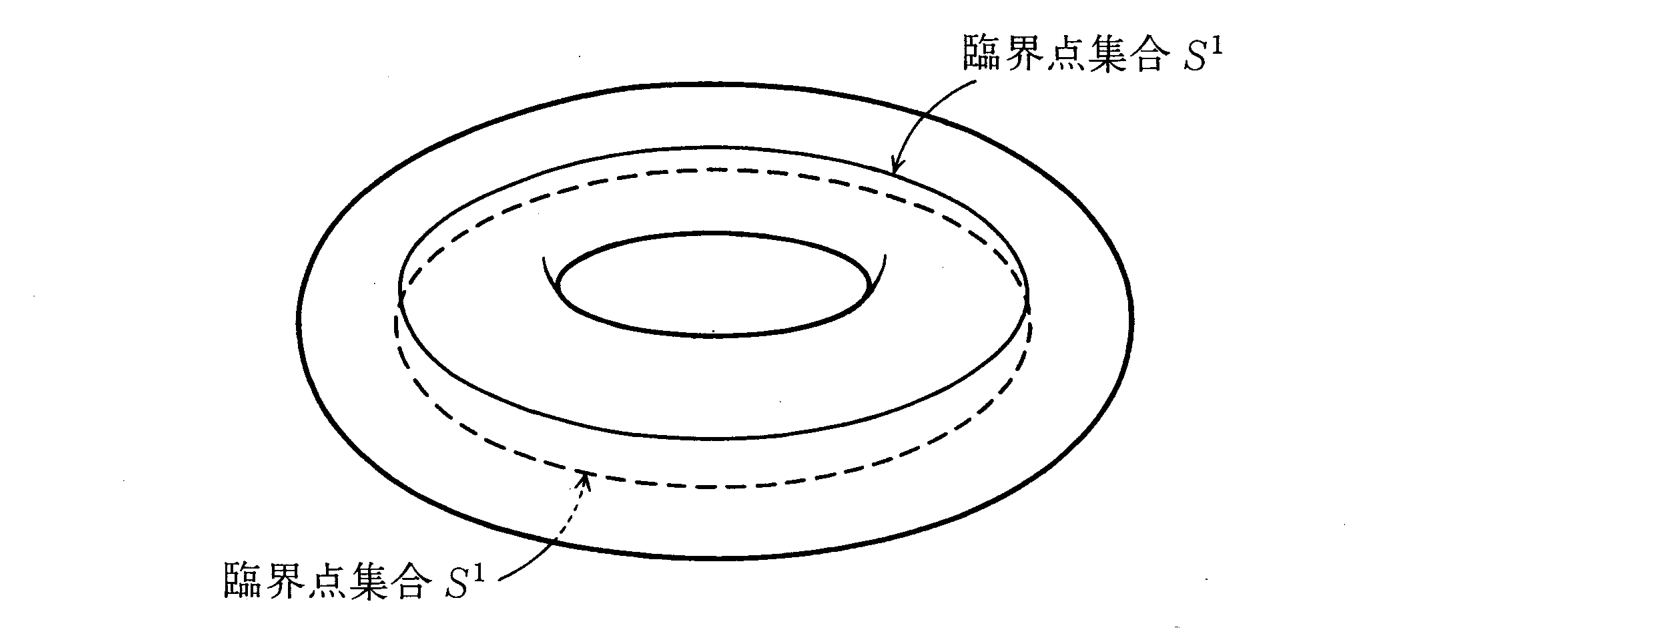
\includegraphics[width=0.62\textwidth]{figures/fig5.2.png}
  \figtitle{5.2}{Bott–Morse 函数 I（原书 p.219）}
\end{figure}

一般地，(5.15) 照原样是有问题的。因为 $\mathcal{M}(R_1,R_2;f)$ 一般带有边界，而用带边流形给出的对应，不能定义为同调元素之间的映射。

\begin{example}{5.79}
  考虑图 5.3 的 Bott–Morse 函数。临界点集合有 5 个连通分支。其中 4 个是单点，1 个是 $S^1$。在由单点构成的连通分支中，2 个的 Morse 指数为 2，记作 $p_1,p_2$；其余 2 个的 Morse 指数为 1，记作 $q_1,q_2$。$\mathcal{M}(p_i,q_j;f)$ 由单点构成，$\mathcal{M}(q_j,S^1;f)$ 由 2 点构成。设后者这 2 条积分曲线与 $S^1$ 的交点为 $r_{j,1},r_{j,2}$。于是 $\mathcal{M}(p_1,S^1;f)$ 是两条线段之和，$\ev_+$ 的像为 $\overline{r_{1,1}r_{2,1}}$ 与 $\overline{r_{1,2}r_{2,2}}$。因此，从 $p_1$ 出发按 (5.15) 计算，会出现一条并非 $S^1$ 上闭链的链。
\end{example}

要解决刚才指出的问题，就必须把构造直接做到取同调之前的链复形上。

% [原文 p.220]
\begin{figure}[htbp]
  \centering
  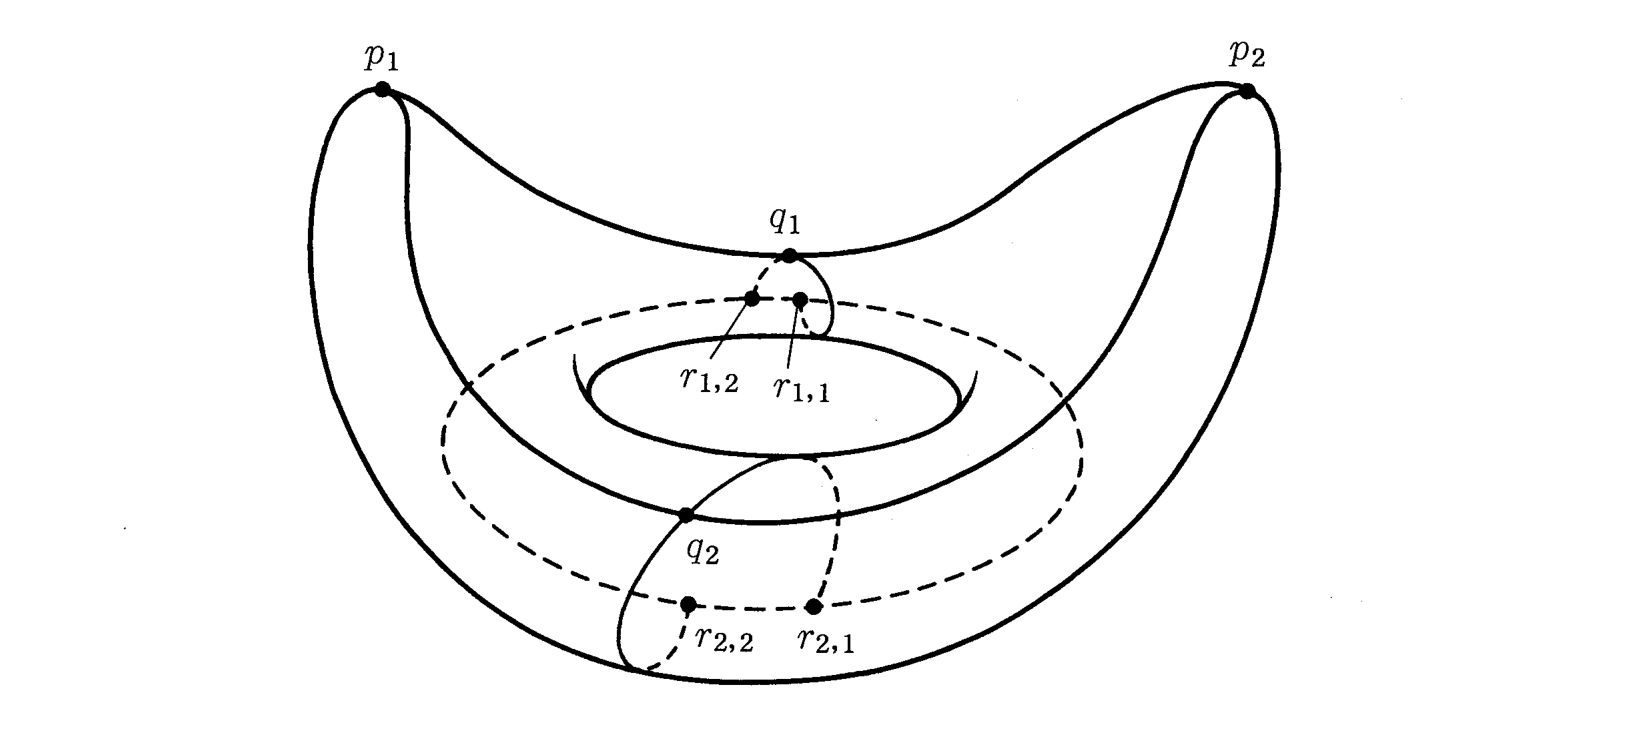
\includegraphics[width=0.66\textwidth]{figures/fig5.3.png}
  \figtitle{5.3}{Bott–Morse 函数 II（原书 p.220）}
\end{figure}

% [Tutor Note: 图 5.3 中 $p_1,p_2$ 是指数 2 的单点临界点，$q_1,q_2$ 是指数 1 的单点临界点，中间的虚线圆与实线圆是两个 $S^1$ 临界点集合。指数 2 的点出发的梯度线落到 $q_j$，再沿 $q_j$ 的两条线打到 $S^1$，故在 $S^1$ 上留下两条线段（例 5.79 中的 $\overline{r_{1,1}r_{2,1}}$ 等），这正是 (5.15) 失效的几何来源。]

\begin{remark}{5.80}
  Austin–Braam [26] 用 Bott–Morse 理论研究了等变上同调，但用的是微分形式（de Rham 上同调）。在 de Rham 上同调中，与 (5.15) 相当的是微分形式的拉回与纤维积分的合成
  \begin{equation}
    u\mapsto \ev_{+,i,j\,!}\circ\ev^{*}_{-,i,j}(u) \tag{5.16}
  \end{equation}
  （$u$ 是 $R_i$ 上的微分形式）。为了处理纤维积分 $\ev_{+,i,j\,!}$，Austin–Braam 加了“$\ev_{+,i,j}$ 是纤维丛”这一假设。该假设在与等变上同调相关的状况下成立，但一般不成立（例 5.79）。而且，要证明所得谱序列不依赖于 Bott–Morse 函数，仍然必须去掉这一假设。从与本节相同的立场讨论等变上同调，见 [382]。

  一旦去掉 $\ev_{+,i,j}$ 是纤维丛的假设，即使从光滑的微分形式 $u$ 出发，(5.16) 也只会成为流（current），不再光滑。一般不存在流之间的拉回映射，因此要用流来正当化 (5.16)，就必须慎重选择把流扩充到何种程度。下面用所谓几何链来回避这一困难；而几何链的横截正则性讨论，与上述“把所考虑的流扩充到适当之处”的问题等价。
\end{remark}

\begin{definition}{5.81}
  $(P,\psi)$ 是流形 $X$ 的 $k$ 维几何链\footnote{几何链这一概念由 Gromov 在 [158] 中为与此处不同的目的引入。}（geometric chain），是指以下条件得到满足。

  % [原文 p.221]
  \begin{enumerate}[label=(\arabic*),leftmargin=2.4em,itemsep=1pt,topsep=2pt]
    \item $P$ 是 $k$ 维单纯复形。$P_i$ 表示其 $i$ 骨架（$i$-skeleton，即 $i$ 维以下单形之和）。
    \item 存在 $P$ 的 $k-1$ 维部分复形 $\partial P$。
    \item $P-P_{k-2}$ 是（带边的）组合流形。
    \item $\partial P-P_{k-3}$ 是 $P-P_{k-2}$ 的边界。
    \item $\psi\colon P\to X$ 连续，且到 $P-P_{k-2}$ 上的限制是分段光滑的。
  \end{enumerate}
\end{definition}

令 $\partial(P,\psi)=(\partial P,\psi)$。则 $\partial\partial=0$。

\begin{definition}{5.82}
  当 $(P_{\pm,i},\psi_{\pm,i})$ 是次数 $k$ 的几何链时，把
  \[
    (P_{+,1},\psi_{+,1})-(P_{-,1},\psi_{-,1})\sim(P_{+,2},\psi_{+,2})-(P_{-,2},\psi_{-,2})
  \]
  定义为：对任意微分 $k$ 形式 $u$，都有
  \[
    \int_{P_{+,1}}\psi^{*}_{+,1}u-\int_{P_{-,1}}\psi^{*}_{-,1}u
    =\int_{P_{+,2}}\psi^{*}_{+,2}u-\int_{P_{-,2}}\psi^{*}_{-,2}u .
  \]
  把 $(P_+,\psi_+)-(P_-,\psi_-)$ 这样的形式差全体按关系 $\sim$ 作商，所得记作 $S_*(X;\Z)$。$S_*(X;\Z)$ 显然构成链复形。
\end{definition}

下面的引理是显然的。

\begin{lemma}{5.83}
  $S_*(X;\Z)$ 的同调与 $X$ 的同调一致。
\end{lemma}

这里用的是上同调的语言，所以把余维数 $k$ 的几何链看作 $k$ 维余链（cochain）。另外，把 $S_k(X;\Z)$ 写作 $S^{\dim X-k}(X;\Z)$。

现在考虑对应 $\ev_-\colon\mathcal{M}(R_i,R_j;f)\to R_i$ 与 $\ev_+\colon\mathcal{M}(R_i,R_j;f)\to R_j$。对 $R_i$ 的几何链 $(P,\psi)$，用纤维积定义 $R_j$ 的几何链 $\delta_{j-i}(P,\psi)$ 为
\begin{equation}
  \delta_{j-i}(P,\psi)=\bigl(P_\psi\times_{\ev_{-,i,j}}\mathcal{M}(R_i,R_j;f),\ \ev_{+,i,j}\bigr). \tag{5.17}
\end{equation}
当然，为使 (5.17) 有定义，$P$ 与 $\mathcal{M}(R_i,R_j;f)$ 必须在 $R_i$ 上横截。(5.17) 即 (5.15) 在链复形层面的对应物。

所需横截正则性的引理如下。

\begin{lemma}{5.84}
  在临界点之外把 $f$ 稍作扰动，则存在 $R_i$ 的几何链的可数集合 $\mathcal{X}_i$，使下述性质成立。
  \begin{enumerate}[label=(\arabic*),leftmargin=2.4em,itemsep=1pt,topsep=2pt]
    \item 对任意 $(P,\psi)\in\mathcal{X}_i$，$\psi\colon P\to R_i$ 与 $\ev_{-,i,j}\colon\mathcal{M}(R_i,R_j;f)\to R_i$ 横截（特别地，(5.17) 有定义）。
    \item 对 $(P,\psi)\in\mathcal{X}_i$，$\delta_{j-i}(P,\psi)$ 与 $\mathcal{X}_j$ 的某个元在定义 5.82 的意义下同值。
    \item 由 $\mathcal{X}_i$ 的元生成的 $S^*(R_i;\Z)$ 的部分复形 $S^*_0(R_i;\Z)$ 的上同调，就是 $R_i$ 的上同调。
  \end{enumerate}
\end{lemma}

% [原文 p.222]
引理 5.84 的证明，是横截性定理与 Baire 范畴定理（category theorem）的标准应用。本书从略。

\begin{definition}{5.85}
  令 $CF^k(X;f)=\bigoplus_i S^{k-\mu(i)}_0(R_i;\Z)$。与通常的边界算子 $\delta_0$ 及 (5.17) 的 $\delta_{j-i}(P,\psi)$ 合起来，定义 $\hat\delta=\sum_i\delta_i$。
\end{definition}

\begin{remark}{5.86}
  严格说来必须注意符号。要凑准符号，多少需要一些关于纤维积定向的讨论。本书省略符号的讨论。参见 [117]。
\end{remark}

\begin{theorem}{5.87}
  $\hat\delta\hat\delta=0$。
\end{theorem}

证明需要关于 $\mathcal{M}(R_i,R_j;f)$ 紧化的讨论。也就是说，需要下面的引理。

\begin{lemma*}{5.88}
  $\mathcal{M}(R_i,R_j;f)$ 可紧化为带角流形 $C\mathcal{M}(R_i,R_j;f)$，其边界 $\partial C\mathcal{M}(R_i,R_j;f)$ 是下式的纤维积之和。
  \begin{equation}
    \bigcup_{i<k<j}\mathcal{M}(R_i,R_k;f)_{\ev_{+,i,k}}\times_{\ev_{-,k,j}}\mathcal{M}(R_k,R_j;f). \tag{5.18}
  \end{equation}
\end{lemma*}

\begin{proof}
  证明与引理 5.24、5.28 类似。设 $\gamma_a\in\mathcal{M}(R_i,R_j;f)$ 是发散列。用 $f(\gamma_a(m_a(s)))=s$ 定义 $m_a$。与引理 5.24、5.28 同样，可知存在 $f(R_i)=r_0<\cdots<r_B=f(R_j)$ 与 $\tau_{a,b}$，使 $s\mapsto m_a(s)+\tau_{a,b}$ 在 $(r_b,r_{b+1})$ 上内闭一致收敛。又，不妨设 $s=r_b,r_{b+1}$ 时 $s\mapsto m_a(s)+\tau_{a,b}$ 发散到 $-\infty,+\infty$。令 $\gamma_{a,b}(t)=\gamma_a(t-\tau_{a,b})$。不妨设 $\gamma_{a,b}$ 内闭一致收敛。把其极限记作 $\gamma_{\infty,b}$。

  由引理 3.19，存在 $k_{b,-},k_{b,+}$ 使 $\gamma_{\infty,b}\in\mathcal{M}(R_{k_{b,-}},R_{k_{b,+}};f)$。

% [原文 p.223]
  于是
\[
\lim_{t\to\infty}f(\gamma_{\infty,b}(t))=r_{b+1},\qquad
\lim_{t\to-\infty}f(\gamma_{\infty,b}(t))=r_b .
\]
故由引理 3.19 的证明，
\[
\mathrm{dist}\bigl(\gamma_{\infty,b}(\infty),\gamma_{\infty,b+1}(-\infty)\bigr)
\le C\Bigl(\lim_{t\to-\infty}\sqrt{f(\gamma_{\infty,b+1}(t))}
-\lim_{t\to\infty}\sqrt{f(\gamma_{\infty,b}(t))}\Bigr)\le 0 .
\]
因此 $\gamma_{\infty,b}(\infty)=\gamma_{\infty,b+1}(-\infty)$。从而 $k_{b,+}=k_{b+1,-}$，重新把这个指标记作 $k_b$，则诸 $\gamma_{\infty,b}$ 给出纤维积
\[
\mathcal{M}(R_{k_i},R_{k_1};f)_{\ev_{+,i,k_1}}
\times_{\ev_{-,k_1,k_2}}\cdots^{\ev_{+,k_{B-2},k_{B-1}}}
\times_{\ev_{-,k_{B-1},k_j}}\mathcal{M}(R_{k_{B-1}},R_j;f)
\]
的元（图 5.4）。于是 $\partial C\mathcal{M}(R_i,R_j;f)$ 含于 (5.17) 之中。反之，证明 (5.17) 的元对应于 $\partial C\mathcal{M}(R_i,R_j;f)$ 的元，则是粘合（gluing）的讨论。
\end{proof}
% [Tutor Note: 上式第一个因子按图 5.4 有 $R_i=R_{k_0}$，第一个求值映射也记为 $\ev_{+,i,k_1}$；作者对左端点的指标混用 $i$ 与 $k_0$，读者对照图 5.4 即可对上。]

\begin{figure}[htbp]
  \centering
  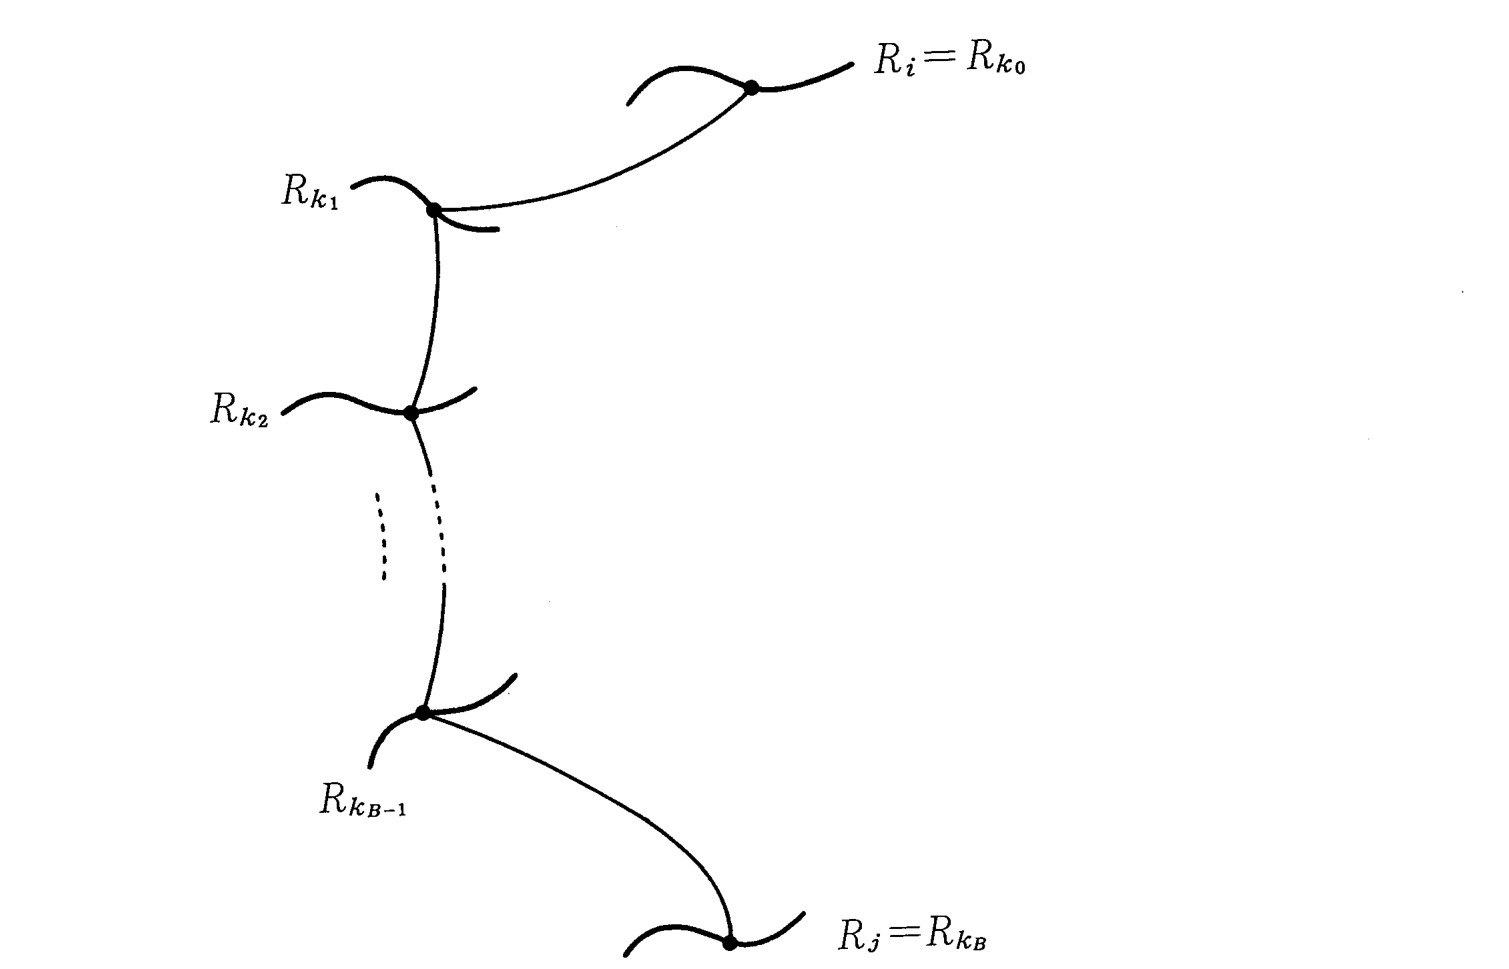
\includegraphics[width=0.56\textwidth]{figures/fig5.4.png}
  \figtitle{5.4}{向许多轨道的分裂（原书 p.223）}
\end{figure}

% [Tutor Note: 图 5.4 画的是发散列在 $f$ 的各个临界值处逐段断开：每一段 $\gamma_{\infty,b}$ 连接 $R_{k_{b-1}}$ 与 $R_{k_b}$，拼起来就是 (5.18) 中那条长长的纤维积。作者把这样断开的极限轨道称为“向许多轨道的分裂”。]

下面完成定理 5.87 的证明。由引理 5.88，
\[
  \resizebox{0.97\linewidth}{!}{$\begin{aligned} \delta\bigl(P_\psi\times_{\ev_{-,i,j}}\mathcal{M}(R_i,R_j;f)\bigr) &=\pm(\delta P)_\psi\times_{\ev_{-,i,j}}\mathcal{M}(R_i,R_j;f)\\ &\quad+\sum_{i<k<j}\pm P_\psi\times_{\ev_{-,i,k}}\mathcal{M}(R_i,R_k;f)_{\ev_{+,i,k}} \times_{\ev_{-,k,j}}\mathcal{M}(R_k,R_j;f) . \end{aligned}$}
\]
这表示

% [原文 p.224]
\[
\delta\delta_{j-i}=\pm\delta_{j-i}\delta+\sum_{k<j-i}\pm\delta_k\delta_{j-i-k},
\]
即 $\hat\delta\hat\delta=0$。

\begin{definition}{5.89}
  $CF^k(X;f)$ 的滤过定义为
  \[
    \mathcal{F}_mCF^k(X;f)=\bigoplus_{i\ge m}S^{k-\mu(i)}_0(R_i;\Z).
  \]
  由定义显然有 $\hat\delta\mathcal{F}_mCF^*(X;f)\subset\mathcal{F}_mCF^*(X;f)$。由这个滤过确定的谱序列记作 $E^*_*(X;f)$。
\end{definition}

下面的式子由定义立即得到。
\begin{equation}
  E^k_2(X;f)\cong\bigoplus_jH^{k-\mu(R_j)}(R_j;\Z). \tag{5.19}
\end{equation}

又，$f=0$ 是 Bott–Morse 函数。对 $f=0$，谱序列退化并给出 $H^*(X;\Z)$，这是显然的。因此，要证明定理 3.17，只要证明下面的定理 5.90 即可。

\begin{theorem*}{5.90}
  $(CF^*(X;f),\hat\delta)$ 的同调不依赖于 Bott–Morse 函数 $f$。
\end{theorem*}

\begin{proof}
  设 $f_{\pm\infty}$ 是两个 Bott–Morse 函数。函数族 $f_\tau$ 定义为
  \[
    f_\tau=
    \begin{cases}
      f_{-\infty}, & \tau<-1\text{ 时},\\
      f_{+\infty}, & \tau>+1\text{ 时}.
    \end{cases}
  \]
  设 $f_{\pm\infty}$ 的临界子流形为 $R_{i,\pm}$。对 $\gamma\colon\R\to X$，考虑常微分方程
  \begin{equation}
    \frac{\partial\gamma}{\partial\tau}=\mathrm{grad}_{\gamma(\tau)}f_\tau . \tag{5.20}
  \end{equation}
  把满足 (5.20)、且 $\gamma(-\infty)\in R_{i,-}$、$\gamma(+\infty)\in R_{j,+}$ 的解 $\gamma$ 全体记作 $\mathcal{M}(R_{i,-},R_{j,+};f_\tau)$。（方程 (5.20) 关于 $\tau$ 的平移并非不变，因此 $\mathcal{M}(R_{i,-},R_{j,+};f_\tau)$ 不带有 $\R$ 作用。）

  适当选取 $f_\tau$，可使 $\mathcal{M}(R_{i,-},R_{j,+};f_\tau)$ 成为 $\dim R_{j,+}+\mu(R_{j,+})-\mu(R_{i,-})$ 维流形。又，$\ev_{-;(i,-),(j,+)}\colon\mathcal{M}(R_{i,-},R_{j,+};f_\tau)\to R_{i,-}$、$\gamma\mapsto\gamma(-\infty)$

% [原文 p.225]
  以及 $\ev_{+;(i,-),(j,+)}\colon\mathcal{M}(R_{i,-},R_{j,+};f_\tau)\to R_{j,+}$、$\gamma\mapsto\gamma(\infty)$ 都是光滑映射。

\begin{remark}{5.91}
  $\mu$ 的确定方式有整体相差一个常数的任意性。如下做法可以消除这个任意性。首先，$f\equiv0$ 时 $\mathrm{Cr}(f)=X$，取 $\mu(M)=0$。一般情形取满足 $f_{-\infty}=0$、$f_\infty=f$ 的 $f_\tau$，再按 $\mathcal{M}(X,R_j;f_\tau)$ 的维数为 $\dim R_j+\mu(R_j)$ 来确定 $\mu(R_j)$ 即可。
\end{remark}

下面的引理与引理 5.88 同样证明。

\begin{lemma}{5.92}
  $\mathcal{M}(R_{i,-},R_{j,+};f_\tau)$ 有紧化 $C\mathcal{M}(R_{i,-},R_{j,+};f_\tau)$，其边界是下面两个集合之和。
  \[
    \bigcup_{i<i'}\mathcal{M}(R_{i,-},R_{i',-};f_{-\infty})_{\ev_{+,i,i'}}
    \times_{\ev_{-(i',-),(j,+)}}\mathcal{M}(R_{i',-},R_{j,+};f_\tau),
  \]
  \[
    \bigcup_{j'<j}\mathcal{M}(R_{i,-},R_{j',+};f_\tau)_{\ev_{+(i,-),(j',+)}}
    \times_{\ev_{-,j',j}}\mathcal{M}(R_{j',+},R_{j,+};f_{+\infty}).
  \]
\end{lemma}
% [Tutor Note: 两个边界项分别是“左端断开”与“右端断开”：第一项把出发点从 $R_{i,-}$ 推到更低的 $R_{i',-}$，第二项把终点从 $R_{j,+}$ 降下来。这与引理 5.88 的 $i<k<j$ 型边界是同一件事，只是两端换成了带 $\pm$ 参数的临界子流形。]

定义 $\Phi^{f_\tau}\colon C^*(X;f_{-\infty})\to C^*(X;f_\infty)$。对 $(P,\psi)\in S_{k,0}(R_{i,-})$，定义
\begin{equation}
  \Phi^{f_\tau}_{j-i}(P,\psi)=\bigl(P_\psi\times_{\ev_{-(i',-),(j,+)}}\mathcal{M}(R_{i,-},R_{j,+};f_\tau),\ \ev_{+,j}\bigr) \tag{5.21}
\end{equation}
并令 $\Phi^{f_\tau}=\sum_k\Phi^{f_\tau}_k$。
% [Tutor Note: 原书 (5.21) 中求值映射的下标写作 $(i',-)$，但左因子取的是 $P_\psi\subset R_{i,-}$，按 (5.20) 式的下标约定应为 $(i,-)$；此处疑为承上文第二个边界项的笔误。译文照原样保留。]

\begin{remark}{5.93}
  也许有人会担心 (5.21) 的右边是哪个群里的元。要弄清这一点，可如下讨论。首先证明：$(C^*(X;f),\hat\delta)$ 的同调，在把引理 5.84 的 $\mathcal{X}_i$ 放大时，只要仍满足引理 5.84 的结论，就不改变。实际上，自然的嵌入给出链映射，而考察谱序列便知它在 $E_2$ 上同构；因此在 $E_\infty$ 上也同构。（参见关于谱序列的比较定理，如 [367]。）

  注意到这一点，就可以把 $CF^*(X;f_{+\infty})$ 放大到包含 (5.21) 的左边，从而 $\Phi^{f_\tau}$ 的定义得到正当化。把这些讨论全写出来太费事，下面从简。
\end{remark}

\begin{lemma}{5.94}
  $\Phi^{f_\tau}$ 是链映射。
\end{lemma}

证明可用引理 5.92，与定理 5.87 同样作出。

% [原文 p.226]
要完成定理 5.90 的证明，只需证明合成 $\Phi^{f_{-\tau}}\circ\Phi^{f_\tau}$ 与恒等映射链同伦。令 $f_{\tau,T}$ 为
\[
f_{\tau,T}=
\begin{cases}
  f_{-\infty}, & |\tau|>T\text{ 时},\\
  f_{+\infty}, & |\tau|<T-2\text{ 时},\\
  f_{\tau-1+T}, & -T<\tau<2-T\text{ 时},\\
  f_{-\tau-1+T}, & T>\tau>T-2\text{ 时}.
\end{cases}
\]
（这里 $f_{\tau,T}$ 是把 $\tau\mapsto f_{+\tau}$ 平移 $-T+1$、再与把 $\tau\mapsto f_{-\tau}$ 平移 $T-1$ 所得者拼起来的。）考虑与 (5.20) 同样的常微分方程
\[
\frac{d\gamma}{d\tau}=\mathrm{grad}_{\gamma(\tau)}f_{\tau,T},
\]
把满足边界条件 $\gamma(-\infty)\in R_{i,-}$、$\gamma(\infty)\in R_{j,-}$ 的解 $\gamma$ 全体记作 $\mathcal{M}(R_{i,-},R_{j,-};f_{\tau,T})$（同样不带 $\R$ 作用）。把 $f_\tau$ 稍作平移，不妨设 $\mathcal{M}(R_{i,-},R_{j,-};f_{\tau,T})$ 是 $\dim R_{j,-}+\mu(R_{j,-})-\mu(R_{i,-})$ 维流形。进一步，与引理 5.88 的证明同样可得下面的引理。

\begin{lemma}{5.95}
  $T$ 充分大时，$\mathcal{M}(R_{i,-},R_{j,-};f_{\tau,T})$ 同胚于下面的并集。
  \[
    \bigcup_k\mathcal{M}(R_{i,-},R_{k,+};f_\tau)_{\ev_{+,k}}
    \times_{\ev_{-,k}}\mathcal{M}(R_{k,+},R_{j,-};f_{-\tau}).
  \]
\end{lemma}

由引理 5.95，合成 $\Phi^{f_{-\tau}}\circ\Phi^{f_\tau}$ 由对应
\begin{equation}
  (P,\psi)\mapsto\bigl(P_\psi\times_{\ev_{-,i}}\mathcal{M}(R_{i,-},R_{j,-};f_{\tau,T}),\ \ev_{-,j}\bigr) \tag{5.22}
\end{equation}
给出。我们想证明 (5.22) 与恒等映射链同伦。取充分大的 $T$ 并固定。对 $\rho\in[0,1]$，按
\begin{equation}
  f_{\tau,\rho}=
  \begin{cases}
    f_{-\infty}, & \rho=0\text{ 时},\\
    f_{\tau,T}, & \rho=1\text{ 时},\\
    f_{-\infty}, & |\tau|>2T\text{ 时}
  \end{cases}
  \tag{5.23}
\end{equation}

% [原文 p.227]
的方式选取 $f_{\tau,\rho}\colon M\times S^1\to\R$。考虑常微分方程
\[
\frac{\partial\gamma}{\partial\tau}=\mathrm{grad}_{\gamma(\tau)}f_{\tau,\rho},
\]
把满足边界条件 $\gamma(-\infty)\in R_{i,-}$、$\gamma(\infty)\in R_{j,-}$ 的解 $\gamma$ 全体记作 $\mathcal{M}(R_{i,-},R_{j,-};f_{\tau,\rho})$。

令
\[
\mathcal{M}(R_{i,-},R_{j,-};f_{\tau,\mathrm{para}})=\bigcup_\rho\mathcal{M}(R_{i,-},R_{j,-};f_{\tau,\rho}).
\]
把 $f_{\tau,\rho}$ 稍作平移，不妨设 $\mathcal{M}(R_{i,-},R_{j,-};f_{\tau,\mathrm{para}})$ 是 $\dim R_{j,-}+\mu(R_{j,-})-\mu(R_{i,-})+1$ 维流形。进一步，

\begin{lemma}{5.96}
  $\mathcal{M}(R_{i,-},R_{j,-};f_{\tau,\mathrm{para}})$ 可紧化为 $C\mathcal{M}(R_{i,-},R_{j,-};f_{\tau,\mathrm{para}})$，其边界是下面的并集。
  \[
    \mathcal{M}(R_{i,-},R_{j,-};f_{\tau,1})\cup-\mathcal{M}(R_{i,-},R_{j,-};f_{\tau,0})
  \]
  \[
    \cup\bigcup_\rho\bigcup_k\mathcal{M}(R_{i,-},R_{k,-};f_{-\infty})_{\ev_{+,k}}
    \times_{\ev_{-,k}}\mathcal{M}(R_{k,-},R_{j,-};f_{\tau,\rho})
  \]
  \[
    \cup\bigcup_\rho\bigcup_k\mathcal{M}(R_{i,-},R_{k,-};f_{\tau,\rho})_{\ev_{+,k}}
    \times_{\ev_{-,k}}\mathcal{M}(R_{k,-},R_{i,-};f_{-\infty}).
  \]
\end{lemma}
% [Tutor Note: 引理 5.96 边界式的第 3 行末因子原书写作 $\mathcal{M}(R_{k,-},R_{i,-};f_{-\infty})$；按第 2 行的对称形状，这里似应为 $R_{j,-}$。译文照原样保留，读者只需知道该项对应“右端断开”。]

证明与引理 5.88 的证明相同。

考察引理 5.96 中出现的 $\mathcal{M}(R_{i,-},R_{j,-};f_{\tau,0})$。由 (5.23)，$f_{\tau,0}\equiv f_{-\infty}$。因此
\[
\mathcal{M}(R_{i,-},R_{j,-};f_{\tau,0})=\tilde{\mathcal{M}}(R_{i,-},R_{j,-};f_{-\infty})
\]
（右边由定义 5.20 定义）。也就是说，$f_{\tau,0}$ 关于 $\R$ 方向的平移不变，因此带有 $\R$ 作用。$i\neq j$ 时这个作用是有效的。又，映射 $\ev_{-,i},\ev_{+,j}$ 关于 $\R$ 作用不变。由此可得下面的引理。

\begin{lemma*}{5.97}
  设 $i\neq j$，$(P,\psi)\in S^*_0(R_{i,-};\Z)$。此时
  \[
    \bigl(P_\psi\times_{\ev_{-,i}}\mathcal{M}(R_{i,-},R_{j,-};f_{\tau,0}),\ \ev_{+,j}\bigr)
  \]
  与 $0$ 在定义 5.82 的意义下同值。
\end{lemma*}

\begin{proof}
  纤维积 $P_\psi\times_{\ev_{-,i}}\mathcal{M}(R_{i,-},R_{j,-};f_{\tau,0})$ 上存在没有 $\R$ 不动点的作用，且 $\ev_{+,j}$ 关于该作用不变。因此，由 $\ev_{+,j}$ 给出的像，比原本的维数

% [原文 p.228]
  $\dim P-\dim R_{i,-}+\dim R_{j,-}+\mu(R_{j,-})-\mu(R_{i,-})$
  小 $1$。引理由此可得。
\end{proof}

% [Tutor Note: 这个论证是“正维数群作用把像的维数压低”的标准用法：$\R$ 自由作用在纤维积上，故其像的维数至多等于原维数减 1，于是该链可写成退化链，在定义 5.82 的意义下与 0 同值。]

$i=j$ 时 $\mathcal{M}(R_{i,-},R_{i,-};f_{\tau,0})\cong R_{i,-}$。总之，在引理 5.95 的第 2 项中作对应，就得到恒等映射。

% [Tutor Note: 引理 5.95 只有一个并集，并没有“第 2 项”；此处应指引理 5.96 边界式中的第 2 项，即 $-\mathcal{M}(R_{i,-},R_{j,-};f_{\tau,0})$（也就是上面讨论的 $f_{\tau,0}$ 项）。译文照原书 5.95 保留。]

另一方面，引理 5.96 第 1 项中的 $\mathcal{M}(R_{i,-},R_{j,-};f_{\tau,1})$ 就是 $\mathcal{M}(R_{i,-},R_{j,-};f_{\tau,T})$。因此由引理 5.96 得到下面的引理。

令
\[
\Phi_{j-i}(P,\psi)=\Bigl(\bigcup_\rho P_\psi\times_{\ev_{-,i}}\mathcal{M}(R_{i,-},R_{j,-};f_{\tau,\rho}),\ \ev_{+,j}\Bigr),
\]
并令 $\Phi=\sum_i\Phi_i$。

\begin{lemma}{5.98}
  $\Phi^{f_{-\tau}}\circ\Phi^{f_\tau}-1=\hat\delta\circ\Phi\pm\Phi\circ\hat\delta$。
\end{lemma}

由引理 5.98，合成 $\Phi^{f_{-\tau}}\circ\Phi^{f_\tau}$ 与恒等映射链同伦。以上完成了定理 5.90 的证明。
\end{proof}

下面证明定理 3.23。也就是说，设 $f$ 是 $S^1$ 作用的动量映射，证明谱序列退化。设 $i\neq j$，考虑模空间 $\mathcal{M}(R_i,R_j;f)$。（这个模空间已经是按 $\R$ 作用取商所得者。定义 5.33。）$R_i,R_j$ 是动量映射的临界点集合，因而是 $S^1$ 的不动点。又，$f$ 是 $S^1$ 不变的。因此，$\mathcal{M}(R_i,R_j;f)$ 上有 $S^1$ 作用。由于 $i\neq j$，这个作用是有效的。

再者，由定义，$\ev_{-,i}\colon\mathcal{M}(R_i,R_j;f)\to R_i$ 与 $\ev_{+,j}\colon\mathcal{M}(R_i,R_j;f)\to R_j$ 关于 $S^1$ 作用不变。于是与引理 5.97 同样可知 $\delta_{j-i}$ 为 0。即 $\hat\delta=\delta$。由此得到定理 3.23。

最后说明定理 5.74 的证明。把定理 5.90 的证明在无限维情形施行，便知 $HF(M;h)\cong HF(M;0)$。$h=0$ 时，$A_h=A$ 是 Bott–Morse 函数，其临界点集合（为把 $A$ 取成单值而提升到 $\Omega_0(M)$ 的覆盖空间上考虑时）是若干个 $M$ 之和。而且 $h=0$ 沿 $S^1$ 方向为常数，因此是 $S^1$ 不变的。（或者说，它是 $S^1$ 在 $\Omega_0(M)$ 上作用的动量映射。）因此，把定理 3.23 的证明在无限维情形施行，谱序列便退化，$HF(M;0)$ 是 $M$ 的同调的直和，

% [原文 p.229]
这正是定理 5.74 所断言的。

本节只对有限维情形给出了严格证明。基于方案 2、给出定理 5.74（及其向任意辛流形的推广）证明细节的文献并不存在。不过，本节所述与模空间紧化等相关的诸结果，可以通过把 [117] Part II 的讨论从规范理论改写为伪全纯曲线来证明。（实际上，规范理论的情形由于有规范变换的自由度，证明更难。）这样一来，本节的讨论便全部得到正当化。又，[122] 在更一般的拉格朗日子流形的 Floer 同调情形，叙述了基于方案 2 的 Floer 同调计算。

\section{伪全纯圆盘的应用}

\takeaway{本节以伪全纯圆盘为工具：在假设 5.100（$\int_{D^2}\varphi^*\omega=0$）下，伪全纯圆盘与伪全纯球面只能取常值，由此构造拉格朗日子流形的 Floer 上同调 $HF(L_1,L_2)$，并借它证明 Gromov 定理：$\C^n$ 中不存在紧致嵌入的完全拉格朗日子流形。}

把 $\C^n=T^*\R^n$ 看作同一对象，并按注意 4.50 定义 $\C^n$ 的完全拉格朗日嵌入。

\begin{theorem}{5.99}
  （Gromov [159]）$\C^n$ 中不存在嵌入的\footnote{既然写的是“子流形”，似乎不必特意写“嵌入的”；但主要论点是拉格朗日浸入存在而嵌入不存在，所以才特意写“嵌入的”加以强调。}紧致完全拉格朗日子流形。
\end{theorem}

设 $z_i=x_i+\sqrt{-1}y_i$ 为 $\C^n$ 的复坐标，$\omega=\sum dx_i\wedge dy_i$ 为其辛形式，$\theta=\sum y_idx_i$。因 $\omega=-d\theta$，$\theta$ 在拉格朗日子流形上的限制成为闭微分形式，确定 de Rham 上同调类。$L$ 是完全拉格朗日子流形，等价于 $[\theta]=0\in H^1(L;\R)$（命题 4.51）。

定理 5.99 与定理 4.151 合起来，给出大量这样的流形例子：到 $\C^n$ 的拉格朗日浸入存在，但拉格朗日嵌入不存在。（例如可知，单连通流形不能拉格朗日嵌入 $\C^n$。）

% [原文 p.230]
定理 5.99 的证明要用拉格朗日子流形的 Floer 上同调\footnote{Gromov 的证明用了伪全纯圆盘，但与下面的不同。用拉格朗日子流形的 Floer 上同调证明定理 5.99 的想法，笔者是从 Oh 那里听来的。}。关于拉格朗日子流形的 Floer 上同调的一般理论，将在 §6.6 概述。本节只叙述困难相对较少的情形。

首先稍作推广。设 $M$ 为辛流形，$L$ 为其（嵌入的）拉格朗日子流形，作如下假设。

\begin{assumption}{5.100}
  对任意满足 $\varphi\colon D^2\to M$、$\varphi(\partial D^2)\subset L$ 的映射 $\varphi$，都有 $\int_{D^2}\varphi^*\omega=0$。
\end{assumption}

当 $L\subset\C^n$ 且 $[\theta]=0\in H^2(L;\R)$ 时，由 Stokes 定理，假设 5.100 得到满足。
% [Tutor Note: 原书 p.230 此处写作 $[\theta]=0\in H^2(L;\R)$，但 $\theta$ 是 1 形式，其 de Rham 类应属 $H^1$；同书 p.229 正作 $[\theta]=0\in H^1(L;\R)$。疑为笔误，译文照原页保留。]

假设 5.100 满足时，可知对任意 $\varphi\colon S^2\to M$ 都有 $\varphi_*[S^2]\cap\omega=0$。也就是说，在 $\pi_2(M)\to H_2(M)$ 的像上 $[\omega]$ 为 0。由此也可看出，假设 5.100 是相当强的限制。
% [Tutor Note: 这里的 $\cap$ 不是链与链的相交，而是链与形式的配对：$\varphi_*[S^2]\cap\omega=\int_{S^2}\varphi^*\omega=\langle[\omega],\varphi_*[S^2]\rangle$。作者在全书用 $\cap$ 表示这种配对，读到 $[\beta]\cap[\omega]$ 时同样作此理解。]

\begin{lemma*}{5.101}
  对满足假设 5.100 的 $L$，满足 $\varphi\colon D^2\to M$、$\varphi(\partial D^2)\subset L$ 的伪全纯映射 $\varphi$ 只能是常值映射。又，$\varphi\colon S^2\to M$ 的伪全纯映射也只能是常值映射。
\end{lemma*}

\begin{proof}
  对伪全纯映射 $\varphi$，$\int_{D^2}\varphi^*\omega$ 等于能量。因此 $\varphi$ 的能量为 0，$\varphi$ 是常值映射。对 $\varphi\colon S^2\to M$ 也一样，能量为 0，故若伪全纯则为常值映射。
\end{proof}

设 $L_1,L_2$ 是满足假设 5.100 的 $M$ 的拉格朗日子流形。暂且设 $M$ 紧致。$\C^n$ 不紧致，但这一点后面再说明。假设 $L_1$ 与 $L_2$ 横截。下面说明这种情形下拉格朗日子流形的 Floer 上同调的构造。设 $\Lambda'_{\mathrm{nov},\Z_2}$ 为 $\Z_2$ 系数的普遍 Novikov 环。$CF(L_1,L_2)$ 由下式定义。
\[
CF(L_1,L_2)=\sum_{p\in L_1\cap L_2}\Lambda'_{\mathrm{nov},\Z_2}[p].
\]

\begin{theorem}{5.102}
  （Floer [103]）存在 $\delta\colon CF(L_1,L_2)\to CF(L_1,L_2)$，满足下列条件。

  % [原文 p.231]
  \begin{enumerate}[label=(\arabic*),leftmargin=2.4em,itemsep=1pt,topsep=2pt]
    \item $\delta^2=0$。
    \item 把 $\delta$ 的上同调记作 $HF(L_1,L_2)$，则对完全辛同胚 $\phi_i$，有 $HF(L_1,L_2)\cong HF(\phi_1(L_1),\phi_2(L_2))$。
    \item 对完全辛同胚 $\phi$，有 $HF(L,\phi(L))\cong H(L;\Z_2)\otimes\Lambda'_{\mathrm{nov},\Z_2}$。
  \end{enumerate}
\end{theorem}
% [Tutor Note: $L_0=L_1$ 时 $HF(L,L)$ 同构于 $H(L)\otimes\Lambda'_{\mathrm{nov},\Z_2}$（见下文 (3) 的证明）；这个同构是拉格朗日 Floer 理论中定次数与符号的基准点。注意 (3) 要求 $L$ 与 $\phi(L)$ 横截，否则 $CF$ 的生成元无意义。]

\begin{definition}{5.103}
  把 $HF(L_1,L_2)$ 称为拉格朗日子流形的 Floer 上同调。
\end{definition}

Floer 在 [103] 中假定的是 $\pi_2(M;L)=0$，由这个条件可推出假设 5.100。为使定理 5.99 能被导出，我们把假设稍稍减弱了。但只有假设 5.100 时，Floer 上同调的次数完全无法确定。（若假定 $L$ 可定向，则次数可确定到模 2。）

下面说明：若定理 5.102 在 $M=\C^n$ 的情形成立，则定理 5.99 可导出。设 $L\subset\C^n$ 是嵌入的紧致完全拉格朗日子流形。利用 $L$ 紧致，存在完全辛同胚 $\phi$ 使 $\phi(L)\cap L=\emptyset$。于是 $HF(L,\phi(L))=0$。另一方面由 (3)，$HF(L,\phi(L))\cong H(L;\Z_2)\otimes\Lambda'_{\mathrm{nov},\Z_2}\neq0$。矛盾。

下面叙述定理 5.102 的证明。许多部分与周期哈密顿系统的情形共通，故只叙述要点。计算中也要用 $L_0=L_1$ 的情形，故以下假定 $L_0$ 与 $L_1$ 是（比横截更一般的）干净相交\footnote{干净相交情形下拉格朗日子流形的 Floer 同调，在 [309] 中研究过。}。

与环路空间 $\Omega_0M$ 相当的，是下面的空间。
\[
\Omega(L_0,L_1)=\{\ell\colon[0,1]\to M\mid \ell(0)\in L_0,\ \ell(1)\in L_1\}.
\]
其次考虑泛函 $A_h$ 的类似物。在 $\Omega(L_0,L_1)$ 的每个连通分支上选取基点 $\ell_0$。以下为记号简便，把 $\Omega(L_0,L_1)$ 当作连通、且 $\ell_0$ 只确定了一个来写；一般情形按连通分支分别考虑则完全相同。设 $\gamma\in\Omega(L_0,L_1)$，取连接 $\ell_0$ 与 $\ell$ 的道路 $\gamma$（即 $\gamma(0)=\ell_0$、$\gamma(1)=\ell$）。由 $\tilde\gamma(\tau,t)=\gamma_\tau(t)$ 定出 $\tilde\gamma\colon[0,1]\times[0,1]\to M$，

% [原文 p.232]
并且 $\tilde\gamma(\tau,i)\in L_i$（$i=0,1$）成立。多值函数 $A$ 由下式定义。
\begin{equation}
  \mathcal{A}(\ell)=\int_{[0,1]^2}\tilde\gamma^*\omega . \tag{5.24}
\end{equation}

\begin{lemma}{5.104}
  (5.24) 的右边由 $\tau\mapsto\gamma(\tau)$ 的同伦类决定。$dA$ 作为 $\Omega(L_0,L_1)$ 上的（单值）微分 1 形式确定。
\end{lemma}

证明可用 Stokes 定理作出。

给 $M$ 定一个黎曼度量，$\Omega(L_0,L_1)$ 上就确定了度量。考虑 $A$ 关于这个度量的梯度向量场、研究其积分曲线，是周期哈密顿系统情形下的下一步。拉格朗日子流形的情形也一样，粗略计算可知积分曲线方程仍为
\begin{equation}
  \frac{\partial\tilde\gamma}{\partial\tau}+J_M\Bigl(\frac{\partial\tilde\gamma}{\partial t}\Bigr)=0 . \tag{5.25}
\end{equation}

然而，主张“$J_M(\partial\ell/\partial t)$ 是梯度向量场”仍有问题。因为按通常的想法，$\Omega(L_0,L_1)$ 在 $\ell$ 处的切空间应是 $\ell^*TM$ 的截面中、在 0 处属于 $T_{\ell(0)}L_0$、在 1 处属于 $T_{\ell(1)}L_1$ 者全体，而 $-J_M(\partial\ell/\partial t)$ 一般不满足这个边界条件。若从无限维 Morse 理论的角度考虑这一点，就会变难而难以理解。这里不再考虑这个困难，即不再考虑“梯度向量场”，而是直接把“梯度向量场的积分曲线的模空间”定义为方程 (5.25) 的解的模空间\footnote{如前所述，这个构造在定义阶段难以从无限维空间的 Morse 理论直接正当化。定义的正当性无法由无限维 Morse 理论的讨论直接确认，其根据是下面叙述的关于有限维空间上偏微分方程的讨论。}。

在此之前，需要定义“$A$ 的临界点”。若承认“$-J_M(\partial\ell/\partial t)$ 是梯度向量场”这一（存在上述问题的）主张，则梯度向量场为 0 的情形，就是 $\partial\ell/\partial t$ 为 0，即 $\ell(t)\equiv p\in L_0\cap L_1$ 的情形。这一点也暂且不深究，直接作为定义。也就是说，

% [原文 p.233]
\begin{definition}{5.105}
  $\mathrm{Cr}(L_0,L_1)=L_0\cap L_1\subset\Omega(L_0,L_1)$。
\end{definition}

设 $L_0\cap L_1=\bigcup R_i$ 为连通分支分解。$p\in L_0\cap L_1$ 时，把对应的 $\mathrm{Cr}(L_0,L_1)\subset\Omega(L_0,L_1)$ 的元记作 $\ell_p$。

\begin{definition}{5.106}
  把满足下列条件的映射 $\tilde\gamma\colon\R\times[0,1]\to M$ 全体记作 $\tilde{\mathcal{M}}(L_0,L_1;R_i,R_j)$。
  \begin{enumerate}[label=(\arabic*),leftmargin=2.4em,itemsep=1pt,topsep=2pt]
    \item $\tilde\gamma$ 满足方程 (5.25)。
    \item $\tilde\gamma(\tau,0)\in L_0$，$\tilde\gamma(\tau,1)\in L_1$。
    \item 存在 $p\in R_i$、$q\in R_j$，使 $\lim_{\tau\to-\infty}\tilde\gamma(\tau,t)=p$、$\lim_{\tau\to+\infty}\tilde\gamma(\tau,t)=q$。
  \end{enumerate}
  $\R$ 通过 $s\cdot\tilde\gamma(\tau,t)=\tilde\gamma(s+\tau,t)$ 作用于 $\tilde{\mathcal{M}}(L_0,L_1;R_i,R_j)$。把商空间记作 $\mathcal{M}(L_0,L_1;R_i,R_j)$。
\end{definition}

想用模空间 $\mathcal{M}(L_0,L_1;R_i,R_j)$ 仿照 §5.2、§5.3 的构造定义 Floer 上同调，但困难 5.34(1),(2) 在这种情形仍然存在。不过，由于假设 5.100，困难不大，用已述的讨论就足以应付。又，因为引理 5.101，不再需要气泡的解析，讨论得以简化。

为叙述关于横截正则性的主张，先定义线性化方程。$R_i$ 有维数时，$\tau\to\pm\infty$ 处边界条件的设定需要注意。那部分请参见 [117], [122]。这里只叙述 $R_i=\{p\}$、$R_j=\{q\}$ 的情形，即 $L_0$ 与 $L_1$ 横截相交的情形。设 $\tilde\gamma\in\tilde{\mathcal{M}}(L_0,L_1;p,q)$。把 $\tilde\gamma^*TM$ 的 $L^{1,p}$ 级截面 $V$ 中满足边界条件
\[
V(\tau,1)\in T_{\tilde\gamma(\tau,1)}L_1,\qquad V(\tau,0)\in T_{\tilde\gamma(\tau,0)}L_0
\]
者全体记作 $L^{1,p}(\R\times[0,1];\tilde\gamma^*TM;L_0,L_1)$。（$L^{1,p}$ 级截面连续，故边界条件有意义。）又，把 $\tilde\gamma^*TM\otimes\Lambda^{0,1}$ 在 $\R\times[0,1]$ 上的 $L^{0,p}$ 级截面全体记作 $L^{0,p}(\R\times[0,1];\tilde\gamma^*TM\otimes\Lambda^{0,1})$。

$D_{\tilde\gamma}\bar\partial\colon L^{1,p}(\R\times[0,1];\tilde\gamma^*TM;L_0,L_1)\to L^{0,p}(\R\times[0,1];\tilde\gamma^*TM\otimes\Lambda^{0,1})$ 由
\[
D_{\tilde\gamma}\bar\partial(V)=\bar\partial(V)+\mathcal{N}'(V)
\]
定义。$D_{\tilde\gamma}\bar\partial$ 是 Fredholm 算子，其指数只依赖

% [原文 p.234]
于 $\tilde\gamma$ 的同伦类。下面的引理就是横截正则性。其证明比周期哈密顿系统的情形容易。

\begin{lemma}{5.107}
  把 $J_M$ 稍作变动，即可使对任意 $\tilde\gamma\in\tilde{\mathcal{M}}(L_0,L_1;p,q)$，$D_{\tilde\gamma}\bar\partial$ 都是满射。
\end{lemma}

把 $\tilde{\mathcal{M}}(L_0,L_1;p,q)$ 中 $D_{\tilde\gamma}\bar\partial$ 的指数为 $k+1$ 者全体记作 $\tilde{\mathcal{M}}(L_0,L_1;p,q)_k$，再把它按 $\R$ 作用取商记作 $\mathcal{M}(L_0,L_1;p,q)_k$。由引理 5.107 与隐函数定理，$\mathcal{M}(L_0,L_1;p,q)_k$ 是 $k$ 维流形。

对 $[\tilde\gamma]\in\mathcal{M}(L_0,L_1;p,q)_k$，令
\[
\mathcal{E}(\tilde\gamma)=\int_{\R\times[0,1]}\tilde\gamma^*\omega ,
\]
并把满足 $\mathcal{E}(\tilde\gamma)\le E$ 的 $\tilde\gamma$ 的同值类全体记作 $\mathcal{M}(L_0,L_1;p,q;E)_k$。下面两个引理分别是引理 5.42、引理 5.43 的类似物。（暂且仍假定 $L_0$ 与 $L_1$ 横截。）

\begin{lemma}{5.108}
  设假设 5.100 成立。此时把 $J_M$ 稍作变动，$\mathcal{M}(L_0,L_1;p,q;E)_0$ 就成为紧致的。
\end{lemma}

\begin{lemma}{5.109}
  设假设 5.100 成立。此时把 $J_M$ 稍作变动，下列结论成立。$\mathcal{M}(L_0,L_1;p,q;E)_1$ 以 1 维流形 $C\mathcal{M}(L_0,L_1;p,q;E)_1$ 为其紧化，其边界 $\partial C\mathcal{M}(L_0,L_1;p,q;E)_1$ 由下式给出。
\[
  \resizebox{0.97\linewidth}{!}{$\displaystyle \partial C\mathcal{M}(L_0,L_1;p,q;E)_1 =\bigcup_{r\in L_0\cap L_1}\bigcup_{E_1+E_2=E} \partial C\mathcal{M}(L_0,L_1;p,r;E_1)_0\times\partial C\mathcal{M}(L_0,L_1;r,q;E_2)_0 . $}
\]
\end{lemma}

当 $L_0$ 与 $L_1$ 横截时，如下定义定理 5.102 的 $\delta$。
\begin{equation}
  \delta[p]=\sum_{q,\ \tilde\gamma\in\mathcal{M}(L_0,L_1;p,q)_0}T^{\mathcal{E}(\tilde\gamma)}[q]. \tag{5.26}
\end{equation}

由引理 5.108，右边属于 $CF(L_1,L_2)$。定理 5.102 的 (1) 由引理 5.109 推出。(2) 的证明与周期哈密顿系统的情形相同，故省略。在证明 (3) 之前，先说明引理 5.108、5.109 的证明。许多部分与引理 5.42、5.43 相同，故不详述，只说明

% [原文 p.235]
假设 5.100 是如何使用的。

首先，下面的引理与 §2.6 的定理 2.101 同样证明。（必须证明边界附近相当于定理 2.97 的事。这从略。参见 [25] 等。）

\begin{lemma}{5.110}
  对 $\tilde\gamma_i\in\tilde{\mathcal{M}}(L_0,L_1;p,q;E)$，存在 $\R\times[0,1]$ 的有限子集 $\{p_1,\cdots,p_N\}$，使 $\tilde\gamma_i$ 的某个子列在 $\{p_1,\cdots,p_N\}$ 之外内闭一致收敛。
\end{lemma}

引理 5.110 不需要假设 5.100。使用假设 5.100，则更强的结论成立。

\begin{lemma*}{5.111}
  在假设 5.100 之下，对任意序列 $\tilde\gamma_i\in\tilde{\mathcal{M}}(L_0,L_1;p,q;E)$，都存在（在整个 $\R\times[0,1]$ 上）内闭一致收敛的子列。
\end{lemma*}

\begin{proof}
  由引理 5.110，只需证明 $|d\tilde\gamma_i|$ 一致有界。设 $\sup|d\tilde\gamma_i|=C_i$ 发散，并设 $(\tau_i,t_i)$ 处 $|d\tilde\gamma_i|$ 最大。令 $d_i=\min\{1-t_i,t_i\}$，分两种情形。
  \begin{enumerate}[label=(\arabic*),leftmargin=2.4em,itemsep=1pt,topsep=2pt]
    \item $C_id_i$ 发散的情形。
    \item $C_id_i$ 有界的情形。
  \end{enumerate}
  考虑情形 (1)。令 $R_i=C_id_i$，$B(R_i)$ 为 $\C$ 中以原点为中心、半径 $R_i$ 的球，$\varphi_i\colon B(R_i)\to\R\times[0,1]$ 定义为
  \begin{equation}
    \varphi_i(x+\sqrt{-1}y)=\frac{1}{C_i}(x+\tau_i,\ y+t_i). \tag{5.27}
  \end{equation}
  令 $\psi_i=\tilde\gamma_i\circ\varphi_i$。$\psi_i$ 伪全纯且 $C^1$ 范数有界。因此用椭圆型方程的标准估计，可证它有内闭一致收敛的子列。由假设的 (1)，$\lim R_i=\infty$，故 $\psi_i$ 的定义域趋于整个 $\C$。于是取极限得到伪全纯曲线 $\psi\colon\C\to M$。又，
  \begin{equation}
    \int_{\C}\psi^*\omega\le\limsup\int_{B(R_i)}\psi_i^*\omega\le E . \tag{5.28}
  \end{equation}
  故由定理 2.105，$\psi$ 可延拓为从 $S^2$ 出发的伪全纯映射。然而 $\psi$ 在原点处微分的模长为 1，故不是常值映射。矛盾。

% [原文 p.236]
  其次假定 (2)。不妨设 $t_i\le 1-t_i$（$t_i=d_i$）。取子列使 $\lim t_i$ 收敛，把极限记作 $D$。令
\[
D_i=\{(x,y)\mid x^2+y^2\le C_i^2(1-d_i)^2,\ y\ge -C_id_i\}.
\]
(5.27) 定义了 $D_i\to\R\times[0,1]$。$\psi_i=\tilde\gamma_i\circ\varphi_i\colon D_i\to M$ 伪全纯且 $C^1$ 范数有界，故有内闭一致收敛的子列。极限 $\psi$ 的定义域为 $\{(x,y)\mid y\ge -D\}$。又，$\psi(x,-D)\subset L_0$。进一步，原点处微分的模长为 1，故 $\psi$ 不是常值映射。$\{(x,y)\mid y\ge -D\}$ 经双全纯映射 $u$ 移到 $D^2$。不妨设 $u(1)=\infty$。令 $\psi\circ u=\phi$，则 $\phi\colon D^2-\{1\}\to M$ 伪全纯，且 $\phi(\partial D^2-\{1\})\subset L_0$。又，与 (5.28) 同样可证
\begin{equation}
  \int_{D^2}\phi^*\omega\le E<\infty . \tag{5.29}
\end{equation}
故由下面的定理 5.112，$\phi$ 可延拓为 $D^2\to M$ 的伪全纯映射。这与引理 5.101 矛盾。
\end{proof}

\begin{theorem}{5.112}
  设 $L$ 是 $M$ 的拉格朗日子流形，$p\in\partial D^2$，且 $\phi\colon D^2-\{p\}\to M$ 伪全纯并满足 (5.29)。此时 $\phi$ 可延拓为从 $D^2$ 出发的伪全纯映射。
\end{theorem}

定理 5.112 的证明从略（参见 [289]）。（定理 5.112 不需要假设 5.100。）

从引理 5.101 证明引理 5.108、引理 5.109 的部分，与已述的周期哈密顿系统情形相同，故省略。

转向定理 5.102(3) 的证明。方略与 §5.3 相同，采用 §5.3 开头所述的方案 2。其第 1 段，即把定义扩充到 $L_0,L_1$ 干净相交的情形，以及该情形下定理 5.102(2) 的证明，都与 §5.3 相同。（由于引理 5.111 成立，紧致性的讨论更容易。）出现差异的是第 2 段。即 $L_0=L_1=L$ 的情形的计算。§5.3 的对应部分，即哈密顿函数 $h$ 为 0 时 Floer 上同调的计算（§5.3 末尾给出的定理 5.74 的证明），用到模空间 $\mathcal{M}(M,M;0)$ 的

% [原文 p.237]
$S^1$ 对称性。（$\mathcal{M}(M,M;0)$ 是 $\R\times S^1\to M$ 的能量有限的伪全纯映射全体按 $\R$ 作用取商所得者。这种情形下 $S^1$ 作用来自定义域 $\R\times S^1$ 沿 $S^1$ 方向的旋转。）

本节所考察的拉格朗日子流形情形，考虑的是从 $\R\times[0,1]$ 出发的映射的模空间，因此不存在自然的 $S^1$ 作用。实际上，在没有假设 5.100 的一般情形下，会出现 Floer 上同调 $HF(L,L)$ 与 $L$ 的同调不同的情况（这一事实由 Oh 发现。参见 §6.6 命题 6.247 之后）。

下面用假设 5.100 证明 $HF(L,L)$ 与 $L$ 的上同调一致。设 $L_0=L_1=L$，则 $L\cap L=L$，故 $\mathrm{Cr}(L)=L$，$R_i$ 只有一个，就是 $L$。

\begin{lemma*}{5.113}
  在假设 5.100 之下，$\tilde{\mathcal{M}}(L,L;L,L)$ 由常值映射构成。
\end{lemma*}

\begin{proof}
  考虑 $\tilde{\mathcal{M}}(L,L;L,L)$ 的元 $\R\times[0,1]\to M$。用同构移动定义域，便得到伪全纯映射 $D^2\to M$ 把 $\partial D$ 映入 $L$。由引理 5.101，这是常值映射。
\end{proof}

下面说明引理 5.113 可导出定理 5.102(3)。把 $A$ 提升到由其多值性给出的覆盖空间上，则 $A$ 的临界点集合可看作 $L$ 之和。（$T$ 表示这些连通分支的差异。）定义 Floer 上同调的微分表为 $\hat\delta=\delta_0+\delta_1+\cdots$，其中 $\delta_0$ 是通常的边界算子，$\delta_1$ 以后是用 $\tilde{\mathcal{M}}(L,L;L,L)$ 给出的对应（定义 5.85）。又，$\delta_1$ 以后对应于把某个 $L$ 上的链移到不同连通分支的 $L$ 上的链的映射（参见 §5.3）。由引理 5.113，$\tilde{\mathcal{M}}(L,L;L,L)$ 由常值映射构成，但它们都是 $L$ 之间同一连通分支内的对应，而不是不同连通分支之间的对应。也就是说，它们对 $\delta_1$ 以后没有贡献。因此 $\hat\delta=\delta_0$。由此得到 $HF(L,L)\cong H(L)\otimes\Lambda'_{\mathrm{nov},\Z_2}$。

以上结束了定理 5.102 的证明。

注意先前保留的点，即在 $\C^n$ 这样的非紧流形上同样可以考察伪全纯曲线的模空间。

% [原文 p.238]
\begin{definition}{5.114}
  （Eliashberg–Gromov [95]\footnote{[95] 中还讨论了其他各种类型的凸性，但此处所用 $\C^n$ 的情形有这个定义就足够了。}）设辛流形 $(M,\omega_M)$ 带有与之相容的近复结构 $J_M$。称 $(M,\omega_M,J_M)$ 在无穷远处为凸，是指存在 $M_i\subset M$ 满足下列条件。
  \begin{enumerate}[label=(\arabic*),leftmargin=2.4em,itemsep=1pt,topsep=2pt]
    \item $M_i$ 紧致，$M_i\subset M_{i+1}$，$\bigcup M_i=M$。
    \item $\partial M_i$ 是光滑子流形，且伪凸。
  \end{enumerate}
\end{definition}

显然 $\C^n$ 在无穷远处为凸。另一方面，辛化 $N\times\R$ 在 $\R$ 趋向 $-\infty$ 的一侧无法满足定义 5.114，故在无穷远处不为凸。

设 $M$ 在无穷远处为凸，取如定义中的 $M_i$。设 $M_i^0$ 为 $M_i$ 的内点全体。

\begin{lemma*}{5.115}
  设 $\varphi\colon D^2\to M$ 伪全纯，$L_0,L_1\subset M^0_i$。设 $p,q\in L_0\cap L_1$，令
  \[
    \tilde{\mathcal{M}}'(L_0,L_1;p,q)=\{\tilde\gamma\in\tilde{\mathcal{M}}(L_0,L_1;p,q)\mid \tilde\gamma(\R\times[0,1])\subset M^0_i\},
  \]
  则 $\tilde{\mathcal{M}}'(L_0,L_1;p,q)$ 是 $\tilde{\mathcal{M}}(L_0,L_1;p,q)$ 的闭子集。（拓扑取一致收敛拓扑。）
\end{lemma*}

\begin{proof}
  设结论不成立，$\tilde\gamma$ 属于 $\tilde{\mathcal{M}}'(L_0,L_1;p,q)$ 的闭包但不属于其中。$\tilde\gamma$ 的像含于 $M_i$。存在 $\R\times[0,1]$ 的内点 $p$ 使 $\tilde\gamma(p)\subset\partial M_i$。在 $\tilde\gamma(p)$ 附近把 $M_i$ 表示为 $g(x)\le0$。$g\circ\tilde\gamma$ 是次调和（subharmonic）函数（引理 4.37）。于是由 $g(x)\le0$ 且 $g(p)=0$，得 $g$ 恒等于 0。也就是说，$\tilde\gamma$ 把 $p$ 的邻域映入 $\partial M_i$。另一方面，$\tilde\gamma$ 伪全纯，故 $\tilde\gamma$ 必为常值映射。这与 $\tilde\gamma(0,\tau)\subset L_0$ 矛盾。
\end{proof}
% [Tutor Note: 原书 p.238 末句写作 $\tilde\gamma(0,\tau)\subset L_0$，按定义 5.106 的边界条件应是 $\tilde\gamma(\tau,0)\in L_0$（定义域为 $\R\times[0,1]$，第一个变量是 $\tau$）。译文照原样保留。]

由引理 5.115，可以用 $\tilde{\mathcal{M}}'(L_0,L_1;p,q)$ 代替 $\tilde{\mathcal{M}}(L_0,L_1;p,q)$ 来讨论。于是，由于 $M_i$ 紧致，$M$ 紧致时的讨论可以原样通用\footnote{像这样在无穷远处为凸的辛流形，常常与紧致情形有相同的结论。}。以上结束了定理 5.99、5.102 的证明。

% [原文 p.239]
定理 5.102 除定理 5.99 之外，还有关于拉格朗日子流形相交等的应用。本节余下部分不加证明地叙述若干 Floer 同调关于拉格朗日子流形的应用。下面的定理由定理 5.102 立即得到。

\begin{theorem}{5.116}
  （Floer）设 $L\subset M$ 满足假设 5.100，$\psi\colon M\to M$ 为完全辛同胚，且 $L$ 与 $\psi(L)$ 横截。此时
  \[
    \#(L\cap\psi(L))\ge\sum_k\mathrm{rank}\,H_k(L;\Z_2).
  \]
\end{theorem}

定理 5.116 的同样估计并非对任何 $L$ 都成立。

\begin{example}{5.117}
  设 $\C\subset\CP^1$，$L\subset\C$ 为半径充分小的圆。存在完全辛同胚 $\psi$ 使 $\psi(L)\cap L=\emptyset$，但 $H(S^1;\Z_2)\neq0$。
\end{example}

这个例子意味着，拉格朗日子流形的 Floer 上同调的定义是相当微妙的问题。

拉格朗日子流形的下列条件，是定义 5.13 的类似物。

\begin{definition}{5.118}
  设 $L\subset M$ 为 $n$ 维拉格朗日子流形，$\mu\colon\pi_2(M,L)\to\Z$ 为 Maslov 指数。

  称 $L$ 是\textbf{单调的}，是指存在正数 $\lambda$，使对任意 $\beta\in\pi_2(M,L)$ 都有 $\mu(\beta)=\lambda[\beta]\cap[\omega]$。

  称 $L$ 是\textbf{半正的}，是指不存在满足 $\beta\cap[\omega]>0$ 且 $0>\mu(\beta)\ge3-n$ 的 $\beta\in\pi_2(M,L)$。

  $L$ 的\textbf{最小 Maslov 数}，是指正的 $\mu(\beta)$ 的最小值。$\mu(\beta)$ 恒为 0 时，最小 Maslov 数取为无穷大。
\end{definition}

Oh [290] 在比 Floer 条件更弱的假设下构造了拉格朗日子流形的 Floer 同调，即假设拉格朗日子流形单调且最小 Maslov 数不小于 3。当 $L_1,L_2$ 满足这个假设时，Oh 构造了满足定理 5.102 的 (1),(2) 的 Floer 同调。但 (3) 一般不

% [原文 p.240]
成立（参见注 6.207）。[122] 展开了使 Floer 同调得以定义的障碍理论。其中一部分将在 §6.6 叙述。

关于拉格朗日子流形交点数目的估计，首先研究的是满足下列假设的情形。

\begin{assumption}{5.119}
  存在与 $\omega_M$ 相容的近复结构和映射 $\phi\colon M\to M$，满足下列条件。
  \begin{enumerate}[label=(\arabic*),leftmargin=2.4em,itemsep=1pt,topsep=2pt]
    \item $J_M\circ d\phi=-d\phi\circ J_M$。
    \item $\phi\circ\phi=1$。
    \item $L$ 是 $\{x\in M\mid\phi(x)=x\}$ 的连通分支。
  \end{enumerate}
\end{assumption}

实代数簇（引理 4.9）是满足假设 5.119 的 $L$ 的代表例。

\begin{conjecture}{5.120}
  （Arnold–Givental 猜想）设 $L\subset M$ 满足假设 5.119，$\psi\colon M\to M$ 为完全辛同胚，且 $L$ 与 $\psi(L)$ 横截。此时
  \[
    \#(L\cap\psi(L))\ge\sum_k\mathrm{rank}\,H_k(L;\Z_2).
  \]
\end{conjecture}

设 $(N,\omega_N)$ 为辛流形，$M=N\times N$，$\omega_M=\pi_1^*\omega_N-\pi_2^*\omega_N$。取 $L=N$ 为对角集合，$\phi(x,y)=(y,x)$，则假设 5.119 满足。设 $\bar\psi\colon N\to N$ 为完全辛同胚，则 $\psi(x,y)=(x,\bar\psi(x))$ 也是完全辛同胚。又，$L\cap\psi(L)$ 与 $\psi$ 的不动点一致。这样，Arnold 猜想的与 $\Z_2$ 系数上同调有关的部分，就推广为猜想 5.120。猜想 5.12 与猜想 5.10 也可同样推广。（Givental 的结果 [144] 是这个方向的部分解。）
% [Tutor Note: 原书 p.240 把此处的 $\psi$ 写作 $\psi(x,y)=(x,\bar\psi(x))$，这样的映射与 $y$ 无关，不可能是 $N\times N$ 上的微分同胚；按上下文应为 $\psi(x,y)=(x,\bar\psi(y))$。译文照原样保留。]

下面的结果是猜想 5.120 的部分解，推广了先行者 Oh 等人的结果。

\begin{theorem}{5.121}
  （[122]）对半正的拉格朗日子流形，猜想 5.120 成立。
\end{theorem}

下面两个猜想也与定理 5.99 关系很深。（笔者是从 Oh 那里听到这两个猜想的。）

\begin{conjecture}{5.122}
  设 $L$ 为 $\C^n$ 的拉格朗日子流形，则 Maslov 指数

% [原文 p.241]
  给出的映射 $\mu\colon\pi_1(L)\to\Z$ 的像并不等于 $\{0\}$。
\end{conjecture}

\begin{conjecture}{5.123}
  设 $\phi\colon L\to\C^n$ 为完全拉格朗日浸入，$\phi(L)$ 的自交点全部横截。设自交点数为 $m$，则
  \[
    2m\ge\sum_k\mathrm{rank}\,H_k(L;\Z_2).
  \]
\end{conjecture}

关于 $\C^n$ 的拉格朗日子流形的 Maslov 指数，有 Polterovich [308]、Oh [291]、Viterbo [379] 的结果。

\begin{theorem}{5.124}
  （Polterovich [308]）设 $L$ 为 $\C^n$ 的拉格朗日子流形，则存在 $\beta\in\pi_1(L)$ 使 $3-n\le\mu(\beta)\le n+1$。
\end{theorem}

\begin{theorem}{5.125}
  （Polterovich [308], Oh [291]）设 $L$ 为 $\C^n$ 的单调拉格朗日子流形，则存在 $\beta\in\pi_2(M)$ 使 $1\le\mu(\beta)\le n$。\footnote{$1\le\mu(\beta)\le n+1$ 是 Polterovich 的结果，Oh 把它改进了。}
\end{theorem}

\begin{theorem}{5.126}
  （Viterbo [379]）设 $L$ 为 $\C^n$ 的拉格朗日子流形且与环面微分同胚，则存在 $\beta\in\pi_1(L)$ 使 $1\le\mu(\beta)\le n+1$。\footnote{这个定理的证明没有用到 Floer 同调。}
\end{theorem}

\begin{theorem}{5.127}
  （[122]）设 $L$ 为 $\C^n$ 的拉格朗日子流形，且 $L$ 是 spin 的并满足 $H^2(L;\Q)=0$，则存在 $\beta\in\pi_2(M)$ 使 $1\le\mu(\beta)\le n+1$。
\end{theorem}

伪全纯圆盘在辛几何中的应用还有很多。这里举出 [330], [381]。

此外，Eliashberg [92] 给出了下面定理的用伪全纯圆盘的另一个证明。

\begin{theorem}{5.128}
  （Bennequin [42]）$S^3$ 上存在彼此不同构的接触结构 $\xi_1,\xi_2$，它们作为子向量丛 $\xi_i\subset TS^3$ 是同伦的。
\end{theorem}

定理 5.128 是三维流形接触几何的辛拓扑研究的出发点。关于这一方向的发展，请参照 [93], [97], [226], [364] 等。

% [原文 p.242]
% [本页空白（PDF p.252 亦为空白页），第 5 章正文至此结束。]

\chapterreview{%
本章把 Arnold 猜想的研究工具落在 Floer 同调上，是全书第一次让伪全纯曲线为一个动力系统问题服务。§5.1 从周期哈密顿系统出发陈述 Arnold 猜想，并把它归结为 1 周期轨道的计数；§5.2 用伪全纯曲线与 Novikov 环造出 Floer 链复形 $CF_*(M;h)$，并在半正条件下证明 $\delta\delta=0$；§5.3 借 Bott–Morse 理论证明 $HF(M;h)\cong H(M;\Z)\otimes\Lambda_{\mathrm{nov},\Z}$；§5.4 把整套机器移植到拉格朗日子流形，得到 $HF(L_1,L_2)$，并证明 Gromov 关于 $\C^n$ 中不存在紧致完全拉格朗日子流形的定理。全章的分量在于：它把第 2 章的伪全纯曲线技术真正用到了动力系统上，也为第 6 章的 Gromov–Witten 不变量与同调镜像对称准备了语言；第 4 章备下的 Maslov 指数，到这里才显出用处。

知识脉络有两条。其一是“计数—紧化—定向”的分析线：模空间 $\mathcal{M}(R_i,R_j;f)$ 与 $\mathcal{M}(L_0,L_1;R_i,R_j)$ 的紧化给出谱序列的微分，Bott–Morse 情形用几何链回避“带边流形给出的对应不是同调映射”的困难，拉格朗日情形则用假设 5.100 消去气泡，使紧致性论证大幅简化。其二是“不变量—形变”的代数线：先证同调不依赖 $h$（定理 5.90），再算 $h=0$ 的特例，两步合起来给出与 $H(M)$ 的同构。作者明言 §5.3 只对有限维情形给出严格证明，无限维部分按 [117] 的思路“应当可以”移植；这种“有限维写全、无限维点到”的写法，是本章读法上的关键。

核心结论可归为三条：$HF(M;h)\cong H(M;\Z)\otimes\Lambda_{\mathrm{nov},\Z}$（定理 5.74）；Arnold 猜想在 $\Z_2$ 系数下的相应估计 $\#(L\cap\psi(L))\ge\sum_k\rank H_k(L;\Z_2)$（定理 5.116，猜想 5.120 是它的拉格朗日版推广）；以及 $\C^n$ 中完全拉格朗日子流形的刚性（定理 5.99）。第一条把“计数周期轨道”化归为“算同调”，第二条把交点下界化归为 Betti 数之和，第三条说明辛嵌入远比辛浸入苛刻——三者合起来，正是辛拓扑区别于微分拓扑的地方。

辨析与提醒：Floer“上同调”的名字与 $CF$ 的链复形构造次序相反，初读容易困惑；文中 $CF_k(M;f)$ 与 $CF_k(M;h)$、$CF(L_1,L_2)$ 与 $CF(L_0,L_1)$ 的混用是原书的笔误，译文一律照录并加批注。假设 5.100 比 Floer 原来的 $\pi_2(M;L)=0$ 弱，代价是次数只能确定到模 2；而 §2.5 的半正性条件在这里以 $\mu(\beta)\ge3-n$ 的面貌重新出现，宜对照定义 5.13 阅读。又，§5.4 的模空间用 $\R\times[0,1]$，与周期哈密顿系统的 $\R\times S^1$ 不同，$S^1$ 对称性因而消失，$HF(L,L)\cong H(L)$ 必须另起论证，这正是 §5.4 后半的重心。

评注：作者的取舍很清楚：把解析部分（气泡、横截性、定向）压缩成“参见 [117]”式的交代，只把 Bott–Morse 的代数骨架写全。这样读者能迅速看清同调同构的整体逻辑，却难以据此独立复核 §5.4 的模空间紧化，作者在 §5.3 末尾也承认这一点。与相邻章节的衔接上，§5.2 的 Novikov 环与 §6.2 的 Gromov–Witten 不变量同源，§5.4 的 $HF(L_1,L_2)$ 则在 §6.6 与同调镜像对称重新会合；本章恰好是全书从“存在性定理”过渡到“计数不变量”的接缝。若与第 3 章对读，还能看到同一套 Bott–Morse 论证在有限维（动量映射）与无限维（Floer）两种舞台上的两次登场。
}
% CHUNK ch05b DONE
